\appendix
\section{Derivaciones manuscritas y guía de lectura}\label{app:manual}
Las cinco hojas manuscritas siguientes reúnen la derivación original de $R_p$ y los pasos restantes del modelo. Las cuatro últimas se conservaron en \texttt{hand/02-derivaciones-manuscritas.pdf}, eliminando únicamente la portada vacía del archivo recibido. Los títulos y la lectura de cada hoja se añaden aquí en texto compuesto para relacionar el trabajo a mano con las ecuaciones del artículo; no sustituyen ni modifican los trazos originales.

\subsection{Trabajo, costo, candidato y unicidad global}
La primera hoja parte del avance físico normalizado $Q=eT=1$ para hallar $T(e)=1/e$, y después integra un gasto constante por período en el intervalo $[0,1/e]$. La condición de primer orden mantiene $M$, $F$ y $\kappa$ fijos y selecciona la raíz positiva $q=\sqrt{2F/\kappa}$. La segunda derivada $2F/e^3>0$ justifica un mínimo local; para demostrar que ese punto existe como mínimo global único se sustituye $F=\kappa q^2/2$ y se completa el cuadrado:
\[
K(e;\kappa)-K(q;\kappa)=\frac{\kappa}{2e}(e-q)^2\geq0,
\quad\text{con igualdad únicamente si }e=q.
\]
El resultado utiliza $e>0$, $F>0$ y $\kappa>0$; $M\geq0$ es un supuesto económico pero se cancela en esta comparación.
\begin{center}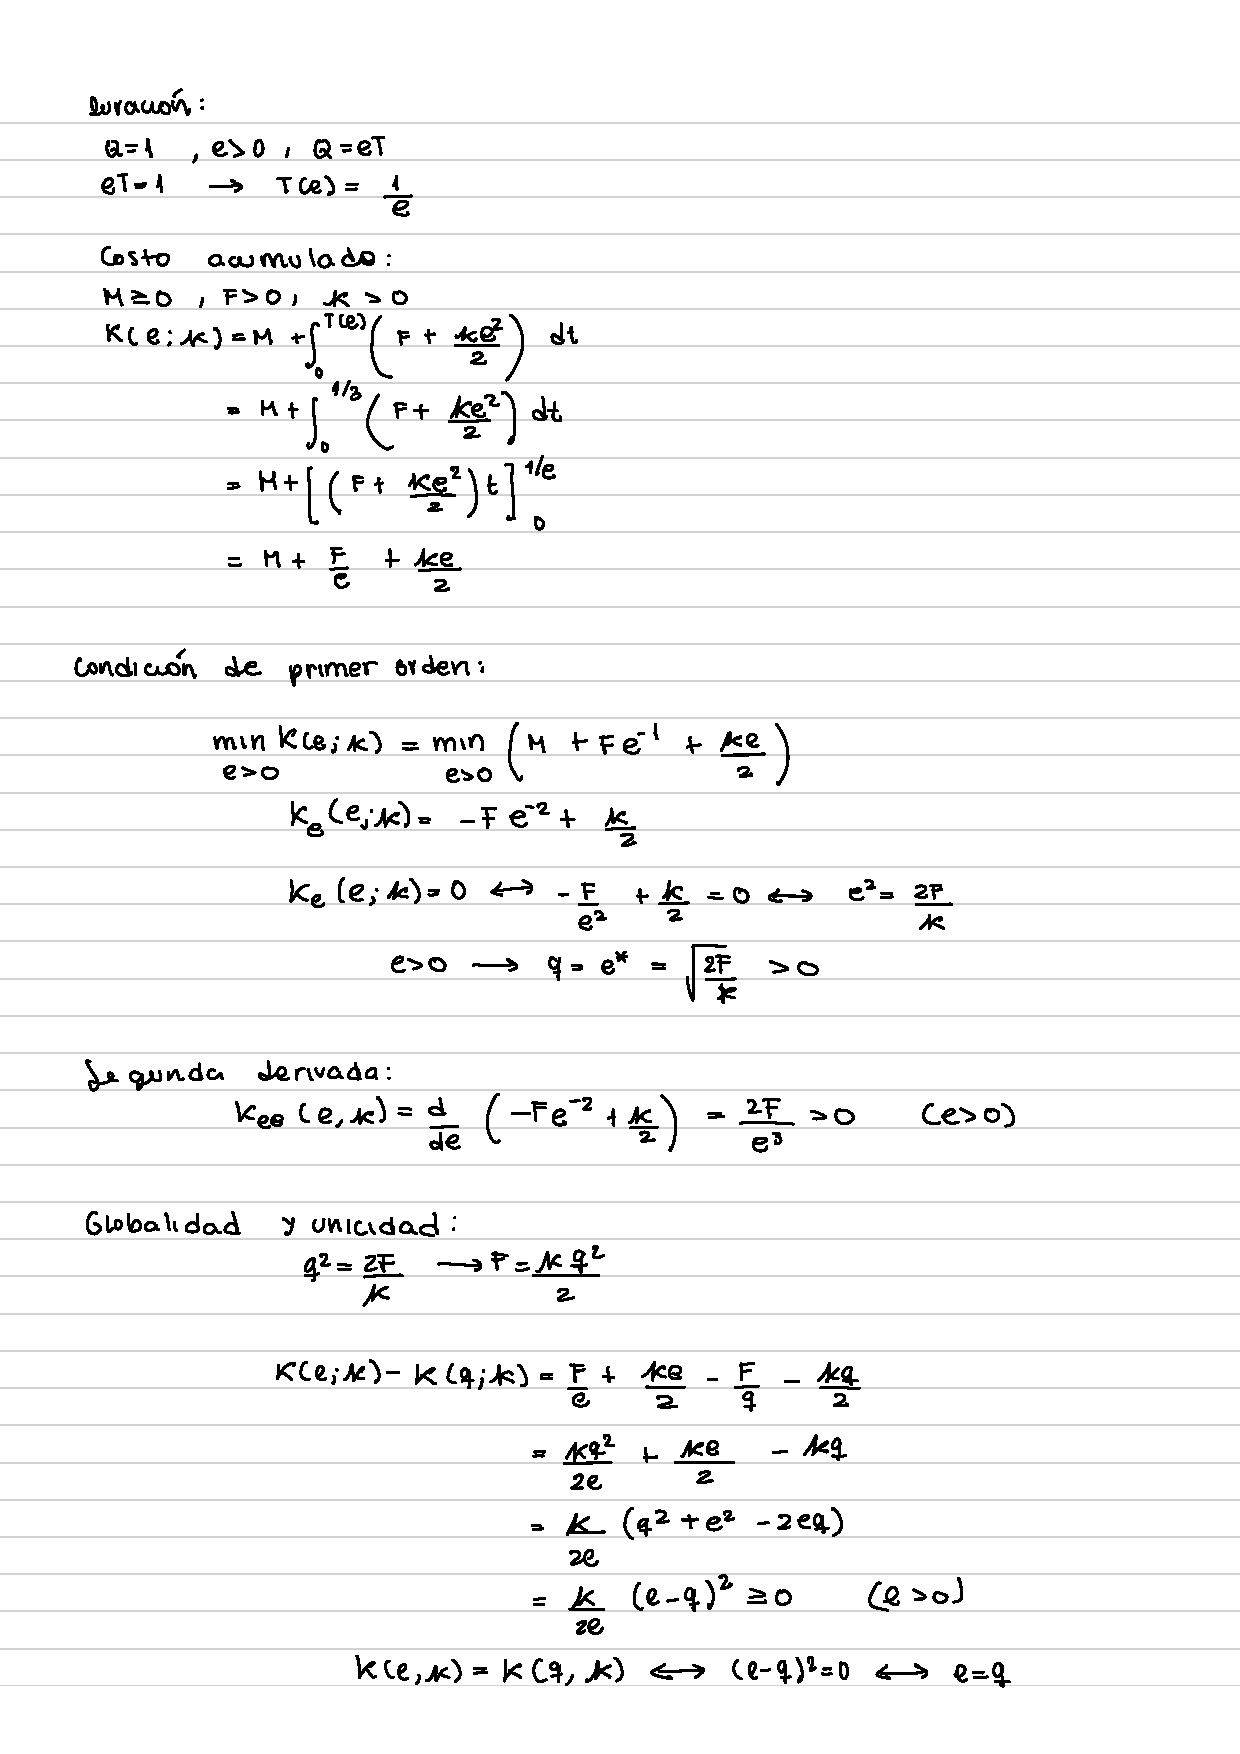
\includegraphics[page=1,width=.96\linewidth,height=.55\textheight,keepaspectratio]{../hand/02-derivaciones-manuscritas.pdf}\end{center}

\clearpage
\subsection{Costo óptimo y signos distritales}
La segunda hoja evalúa $T(q)$ y $K(q;\kappa)$. En el manuscrito, el signo situado entre $K_e(q;\kappa)$ y $0$ puede leerse como una desigualdad; la igualdad que corresponde a la condición de primer orden, y la utilizada en las transformaciones siguientes, es $K_e(q;\kappa)=0$. Al aplicar después la regla de la potencia a $e^*$, $T^*$ y $K^*$ se obtienen signos $(-,+,+)$ respecto de $\kappa$. La regla de la cadena transforma esos signos en los correspondientes a $p$ y $C$, condicionados a $\kappa_p>0$ y $\kappa_C<0$ y a mantener fijos $M$, $F$ y la otra característica distrital.
\begin{center}\includegraphics[page=2,width=.96\linewidth,height=.75\textheight,keepaspectratio]{../hand/02-derivaciones-manuscritas.pdf}\end{center}

\clearpage
\subsection{Tres signos del costo y anticipación parcial}
La tercera hoja aplica la solución óptima dos veces, con $\kV$ en la proyección presupuestaria y $\kA$ al iniciar la ejecución. La cancelación de $M$, el crecimiento estricto de la raíz cuadrada y la monotonía de $\log$ para costos positivos establecen los tres casos de la Proposición~\ref{prop:dos}. Para la extensión, se deriva primero $\kV(\lambda)$ y luego $\KV(\lambda)$; la regla de la cadena para el logaritmo da \eqref{eq:r_lambda}. La comparación requiere el mismo proyecto, alcance, calidad, $M$ y $F$ en ambas etapas.
\begin{center}\includegraphics[page=3,width=.96\linewidth,height=.75\textheight,keepaspectratio]{../hand/02-derivaciones-manuscritas.pdf}\end{center}

\clearpage
\subsection{Convergencia de la previsión y razones de las figuras}
La cuarta hoja usa la identidad $\kA-\kV(\lambda)=(1-\lambda)(\kA-\bar\kappa)$. Para $0\leq\lambda<1$, la Proposición~\ref{prop:dos} fija el signo de $R$; en $\lambda=1$, la coincidencia de las fricciones implica $R=0$, mientras $e^A$ y $\KA$ permanecen constantes. Las razones de intensidad y duración dividen cada solución entre su propia referencia hipotética $e_0$ o $T_0$, calculada con $\bar\kappa$. Esa referencia de la simulación no es la fricción presupuestada $\kV$.
\begin{center}\includegraphics[page=4,width=.96\linewidth,height=.72\textheight,trim=0 350 0 0,clip,keepaspectratio]{../hand/02-derivaciones-manuscritas.pdf}\end{center}

\clearpage
\subsection{Revisión independiente de la derivada respecto de la pobreza}
La hoja anterior de la autora diferencia ambos logaritmos en $R(p)$ mediante la regla de la cadena, de donde $R_p=(\KA)_p/\KA-(\KV)_p/\KV$. Su veredicto es que $\kappa_p^A>0$ por sí sola no determina el signo de $R_p$ cuando $\kappa_p^V$ también puede variar. Si $\kappa_p^V=0$, la positividad de $\kappa_p^A$ sí da $R_p>0$. Así se examina una conclusión demasiado fuerte que podría atribuirse a la asistencia de IA.
\begin{center}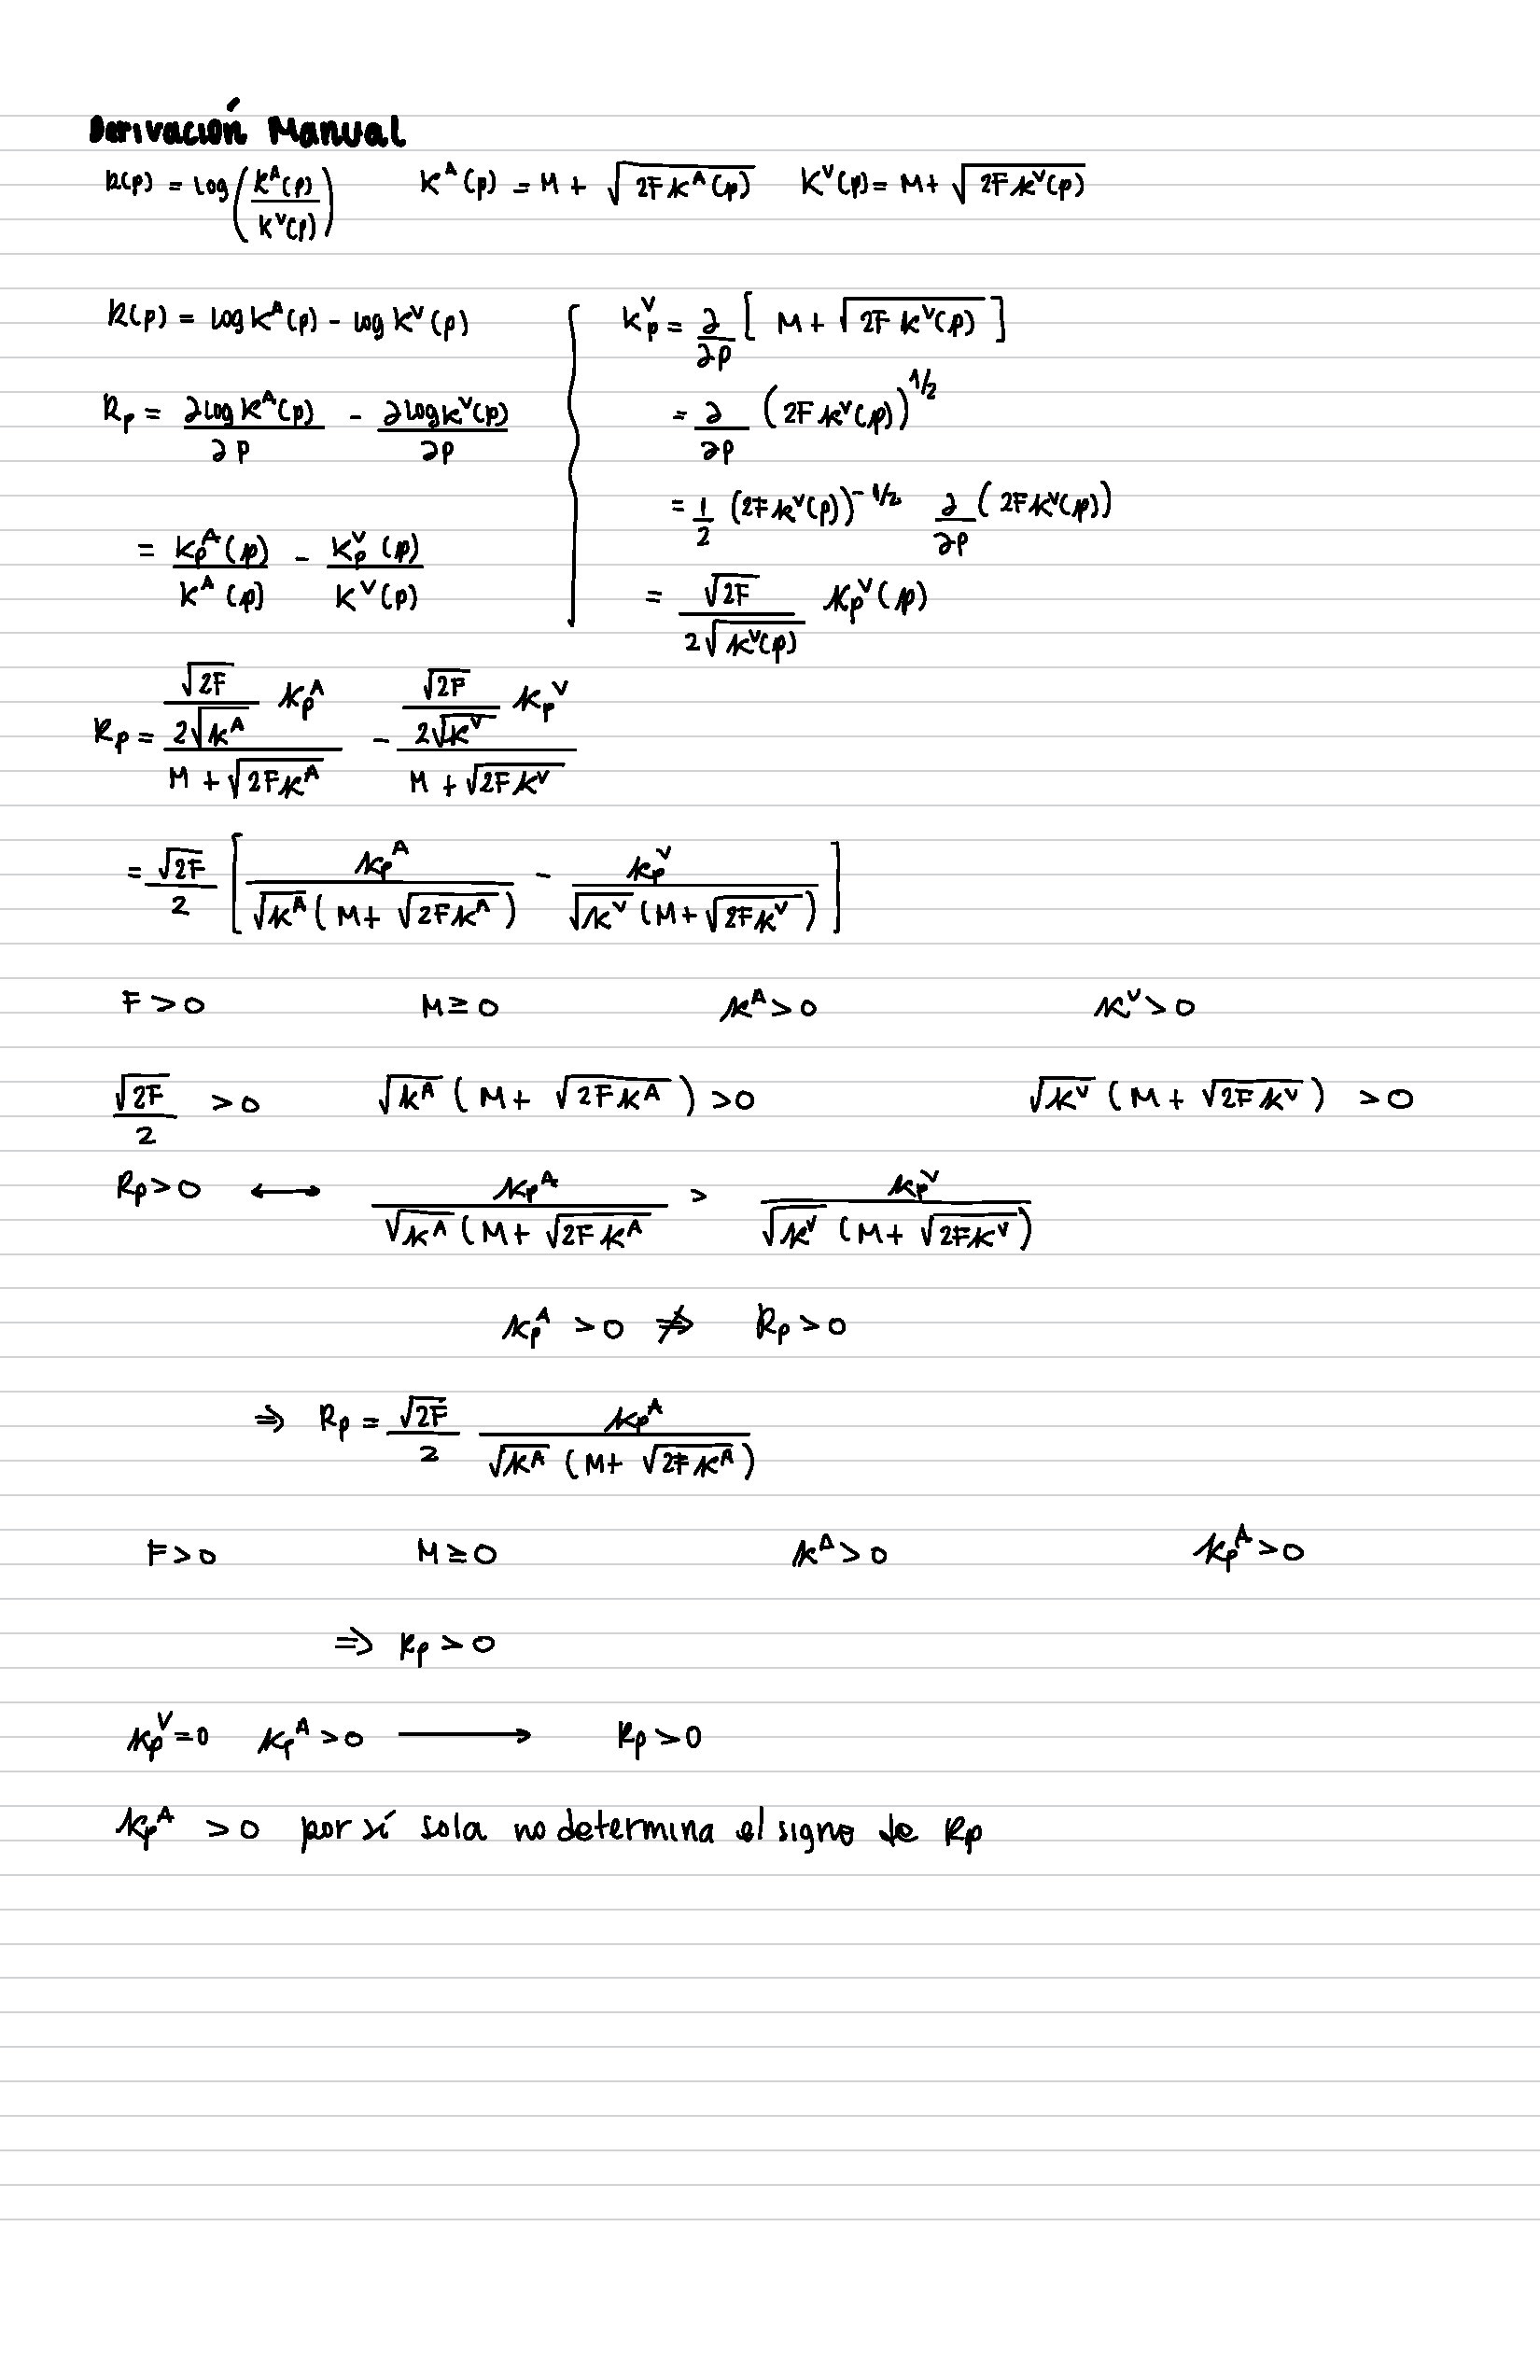
\includegraphics[page=1,width=.96\linewidth,height=.75\textheight,keepaspectratio]{../hand/01-derivacion-manual-Rp.pdf}\end{center}

\clearpage
\section{Correspondencia con la formalización Lean}\label{app:lean}
La formalización disponible se corresponde con la versión del artículo indicada en \texttt{lean/README.md}. Una compilación anterior del archivo \texttt{Proposition1.lean} verificó el mínimo global único; la ejecución del flujo de contribución y las declaraciones de los demás resultados están pendientes de comprobación. La tabla no atribuye a Lean los signos distritales ni el resultado sobre sobrecostos.
\begin{center}
\small
\begin{tabular}{p{.21\linewidth}p{.34\linewidth}p{.34\linewidth}}
\toprule
Resultado del artículo & Declaración y archivo Lean & Estado y alcance \\
\midrule
Proposición 1 & \texttt{MunicipalProject.}\newline\texttt{unique\_global\_minimum} en \texttt{lean/Proposition1.lean} & Mínimo global único compilado anteriormente; duración, costo y signos abiertos. \\
Proposición 2 & --- & Abierta: falta formalizar la equivalencia de los tres signos. \\
Extensión de anticipación & --- & Abierta: falta formalizar $R_\lambda$ y el caso $R(1)=0$. \\
\bottomrule
\end{tabular}
\end{center}


\clearpage
\section{Evaluación de la colaboración con IA}\label{app:ia}
El archivo \texttt{prompts.md} conserva las consultas y respuestas pertinentes en bruto. La tabla separa lo sugerido durante esa colaboración de lo que se admite como resultado de este artículo; el criterio de aceptación es la coincidencia con las hipótesis escritas y la comprobación independiente, no la fluidez de una respuesta.
\begin{center}
\small
\begin{tabular}{p{.21\linewidth}p{.31\linewidth}p{.37\linewidth}}
\toprule
Contribución examinada & Veredicto y razón & Verificación \\
\midrule
Óptimo de intensidad y costo & Aceptada con $F,\kappa>0$ y $e>0$. La condición de primer orden sola no demuestra globalidad. & Identidad cuadrática \eqref{eq:brecha} en el artículo y manuscrito; sustituciones en SymPy y comparación en 3000 casos. \\
Signos distritales & Condicionales, no estimaciones: los signos de $\kappa_p$ y $\kappa_C$ son supuestos estructurales. & Regla de la cadena y manuscrito; contraste de su interpretación con los resultados de \citet{loayza2014}. \\
Sobrecosto siempre que la fricción sea elevada & Rechazada. El nivel absoluto de $\kA$ no fija la diferencia respecto de la previsión. & Resta de costos y tres equivalencias de la Proposición~\ref{prop:dos}; casos positivos, negativos e iguales en \texttt{code/verify.py}. \\
$\kappa_p^A>0$ bastaría para $R_p>0$ & Rechazada si $\kappa_p^V$ puede variar. Ambas derivadas de costos entran en $R_p$. & Hoja manuscrita propia y ecuación \eqref{eq:rp}; comprobación simbólica del código. \\
Mejor anticipación abarata la ejecución & Rechazada bajo la extensión propuesta: $\lambda$ mueve el costo previsto, no $\KA$ con $\kA$ fija. & Derivada \eqref{eq:r_lambda}, límite $R(1)=0$, manuscrito y valores del script. \\
\bottomrule
\end{tabular}
\end{center}
Esta evaluación se limita a las identidades y condiciones de este modelo. La revisión de fuentes literarias y su correspondencia con obras municipales requieren juicio sobre unidades de análisis y sobre el momento en que se fija cada presupuesto; ninguna comprobación algebraica decide esas cuestiones por sí sola.
